\documentclass[a4paper]{article}

\usepackage{parskip}
\usepackage{setspace}
\usepackage{fullpage}
\usepackage{graphicx}
\usepackage{float}

\begin{document}

\title{Planning, Estimating and Tracking}
\author{Andrew Higginson \and Bryan Liu \and Jia Guang Choo \and Emma Hulme \and 
Timothy van Bremen \and Thomas Taylor-Hall}
\date{\today}
\maketitle

\setcounter{table}{0}
\linespread{1.1}

\section{Project Introduction}
As part of the renovation of the William Penney Building on the Sherfield 
walkway, interactive screens are to be installed. Mounted inside the building, four projectors will simultaneously display content onto floor to ceiling glass
panels that are visible to passers-by. Also, an 84-inch 4K resolution touch 
screen is to be mounted by the entrance doors. 

Our project consists of developing an ``App Store" for uploading interactive content and visualisations to be displayed on the four projected screens. Also, we will be developing a playout system to show the content on multiple screens in multiple resolutions.

\section{Understanding User Requirements}

\begin{figure}[H]
  \centering
    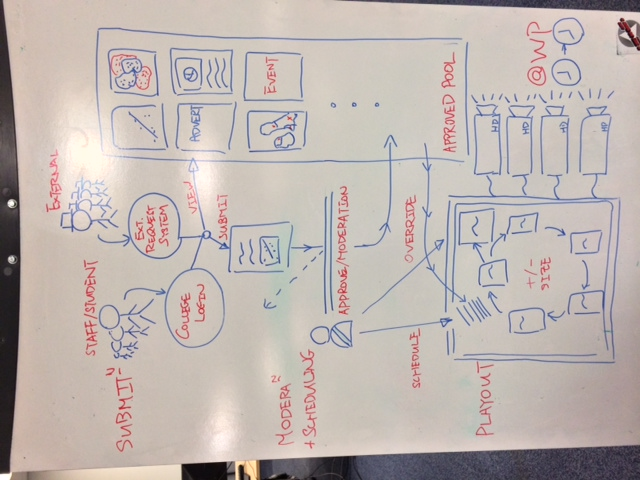
\includegraphics[width = 0.55\textwidth, trim= 0 0.55cm 0 1.4cm, clip]{./planning/userreq.jpg}

  \caption{Initial project specification in a diagram.}
  \label{fig:userreq}
\end{figure}

To better understand user requirements and form the initial backlog of tasks, we held an exploratory meeting with our supervisor, who in this instance plays the role of ``client'' of the 
project.

The ``App Store" is broadly divided into the following three domains:
\begin{itemize}
  \item \textbf{Submission}: allowing users to login, view and submit 
        visualisations/ advertisements
  \item \textbf{Moderation \& Scheduling}: allowing administrators to approve
        and schedule submissions for playout
  \item \textbf{Playout}: allowing scheduled submissions to be projected in
        specified sizes

\end{itemize}



Figure \ref{fig:userreq} illustrates requirements of the system.
The full specification is also available in the appendix.

\section{Task Estimation}
The group is acutely aware that with Computing examinations being held at the
end of term, we could only practically carry out development work until the
first week of December. Furthermore, commitments in other courses mean that 
each team member is only able to devote around 16-20 hours per week to
the project. As a group, we have allowed some leeway for each task in case we run into technical errors. If this is the case, we will communicate between the group and come up with a solution if necessary.

In light of these constraints, we have decided to commit to the following:
\begin{enumerate}
  \item \textbf{To maintain a one-week iteration}: this allows the development team to
        obtain maximum possible feedback from the client/supervisor.
  \item \textbf{To strictly adhere to the original project scope}: while we believe the
        current scope is manageable, we would reject time-consuming items which
        are out of scope before a minimal working system is implemented.
\end{enumerate}


\begin{figure}[h]
  \centering
    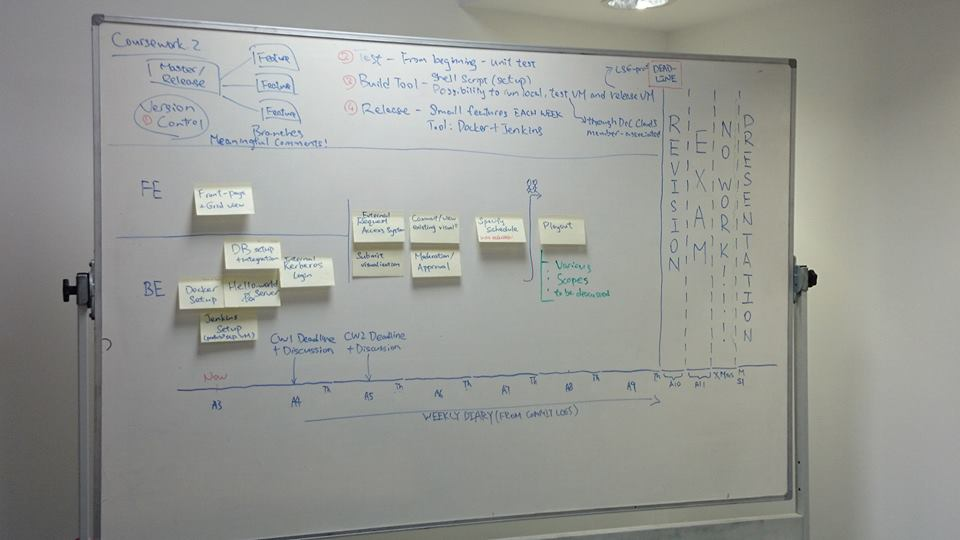
\includegraphics[width = 0.99\textwidth]{./planning/timeline.jpg}
   
  \caption{Project plan with timeline}
  \label{fig:timeline}
\end{figure}


\begin{table}[h]
  \begin{tabular}{c | c | c | c }
    \textbf{Academic Week} & 3 \& 4 (ending 30/10) & 5 (ending 6/11) \\
    \textbf{Iteration/Sprint} & 1 & 2 \\ \hline
    \textbf{Tasks} & Front-page + grid view (FE) & Access request for externals \\
          & Docker Setup (BE)           & Visualisation submission \\
          & Hello-world server (Flask) (BE) & \\
          & MongoDB Setup + Integration (BE) & \\
          & Jenkins Setup at Production VM (BE) & \\
          & Internal Kerberos Login (BE) & \\
  \end{tabular}

  \vspace{30pt}
  \begin{tabular}{c | c | c | c | c}
    \textbf{Academic Week} & 6 (ending 13/11) & 7 (ending 20/11) & 8 (ending 27/11) & 9 (ending 4/12) \\
    \textbf{Iteration/Sprint} & 3 & 4 & 5 & 6 \\ \hline
    \textbf{Tasks} & Comment/view existing visualisations & Scheduling & 
            \multicolumn{2}{c}{Playout} \\
          & Admin moderation/ approval &  \\
  \end{tabular}
  \caption{Project timeline}
  \label{table:timeline}
\end{table}


The resultant plan and timeline shown in figure \ref{fig:timeline} and table
\ref{table:timeline} is a
combination of the plan for next iteration and the release plan, taking account
of the current project scope. Each post-it note either represents a 
concrete task to be completed during the next iteration (towards the left), or
high level themes to be implemented (towards the right). Each line segment at
the bottom represents an iteration ending on Thursday, when the development
team will meet with the client.


Estimates on time required for the tasks were based on their relative size and
time taken for us to complete similar ones in the past. For example, some of us
have implemented a College (Kerberos) Login System well within a week, thus if
it is a size M, we can infer that the team (now double the size) is capable in 
fitting two size M tasks within an iteration. For larger system modules, we
assign a longer period specifically for that task: we expect the scheduling
system (size L) and the entire playout system (size XL) would take us one and
two iteration(s) respectively.


\section{Group organisation} \label{sec:group}
After we established the requirements of the project, each group member stated
which part of the project they would like to work on. We found that there was a
good split of two people that wanted to work on the frontend, two on the backend
server code, and two on the database.

Although this is a good split to initiate work, we realised that the frontend 
aspect of the project may require more work approaching later iterations.
In addition, we  expect that the server code and database should be fully 
implemented within the first four iterations, only requiring minor fixes thereafter.

Therefore, we decided that two people from the backend would move on to creating
the playout software on the dedicated computers; one person would help with the
frontend and the remaining person would apply small fixes and refactors to the
existing server/database code. 


\section{Development Methods \& Project Tracking}
The team has agreed to adopt a mixture of Agile Development Methodologies to
sure our practical need.

For project management, we generally follow the scrum method, adopting the
following characteristics:
\begin{itemize}
  \item \textbf{Roles}: We see Dr. David Birch, our supervisor, as the \textit{Product Owner}
        who provide ideas and feedback for the development. At the same time,
        the team have agreed that Andrew and Bryan should assume the role of
        \textit{Scrum Masters} to facilitate work for the front end and back end respectively.
  \item \textbf{Ceremonies}: Upon the initial meeting, we have established a
        meeting with David each Thursday to review our previous sprint 
        and plan our next sprint. We are to hold a development team
        meeting every Monday (figure \ref{fig:scrum} to update each other 
        on our progress and review work done in past sprints.
  \item \textbf{Artefacts}: We keep our product backlog and iteration backlog on
        Trello as part of our project tracking mechanism (more details
        available in the later part of section).
\end{itemize}


\begin{figure}[ht]
  \centering
    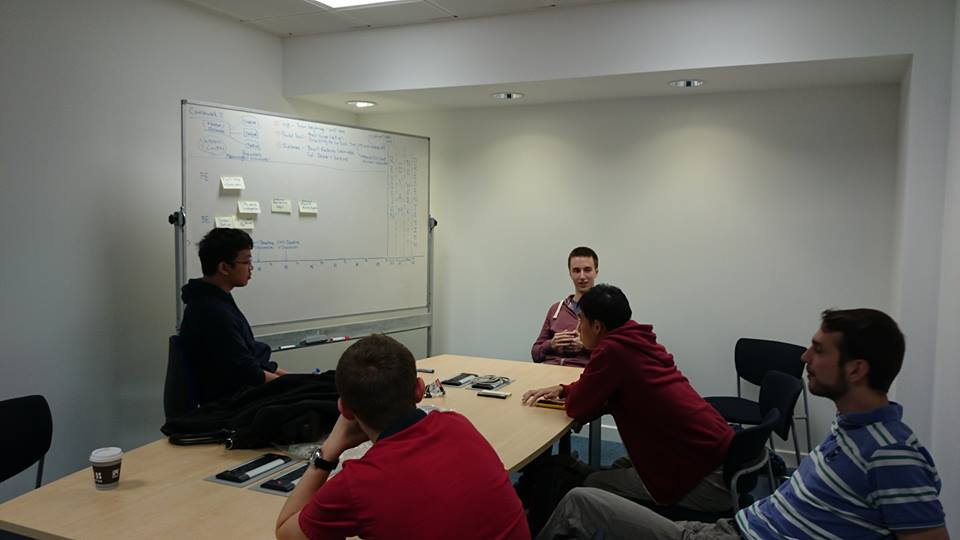
\includegraphics[width = 0.99\textwidth]{./planning/scrum.jpg}
   
  \caption{Half-weekly ``scrum'' (development team meeting).}
  \label{fig:scrum}
\end{figure}

We also integrate a few technical practices inspired by Extreme Programming:
\begin{itemize}
  \item \textbf{Simple Design}: including the use of lightweight technologies that are easy to understand (this was key to our choice of Flask as a backend framework)
  \item \textbf{Pair Programming}: as mentioned in section \ref{sec:group}, we sorted
        ourselves into three pairs, focusing on frontend (FE), backend (BE) and database (DB) work.
        Such a practice allows continuous development on all divisions without
        being affected by instances in which a member is required to temporarily shift his or her
        focus from the project to other coursework/tests.
  \item \textbf{Test-driven Development}: during development, we will constantly be writing small tests to make sure individual features are working as expected before we move on to the next feature.

\end{itemize} 

Finally, to keep track on the group's progress, we use an electronic task
board on Trello (see figure \ref{fig:trello}). Here we can assign ourselves (and others) specific tasks and a general due date. Trello allows us to see what the other members of the group are doing and when a feature is expected to be completed. We can also easily add photos and checklists to see how the project is forming. We decided to use Trello as a physical story-board is not feasible. As well as Trello, we will constantly be communicating personally in labs, online via messaging services, and regular stand-ups in a meeting room. This development process follows the Kanban methodology.

\begin{figure}[ht]
  \centering
    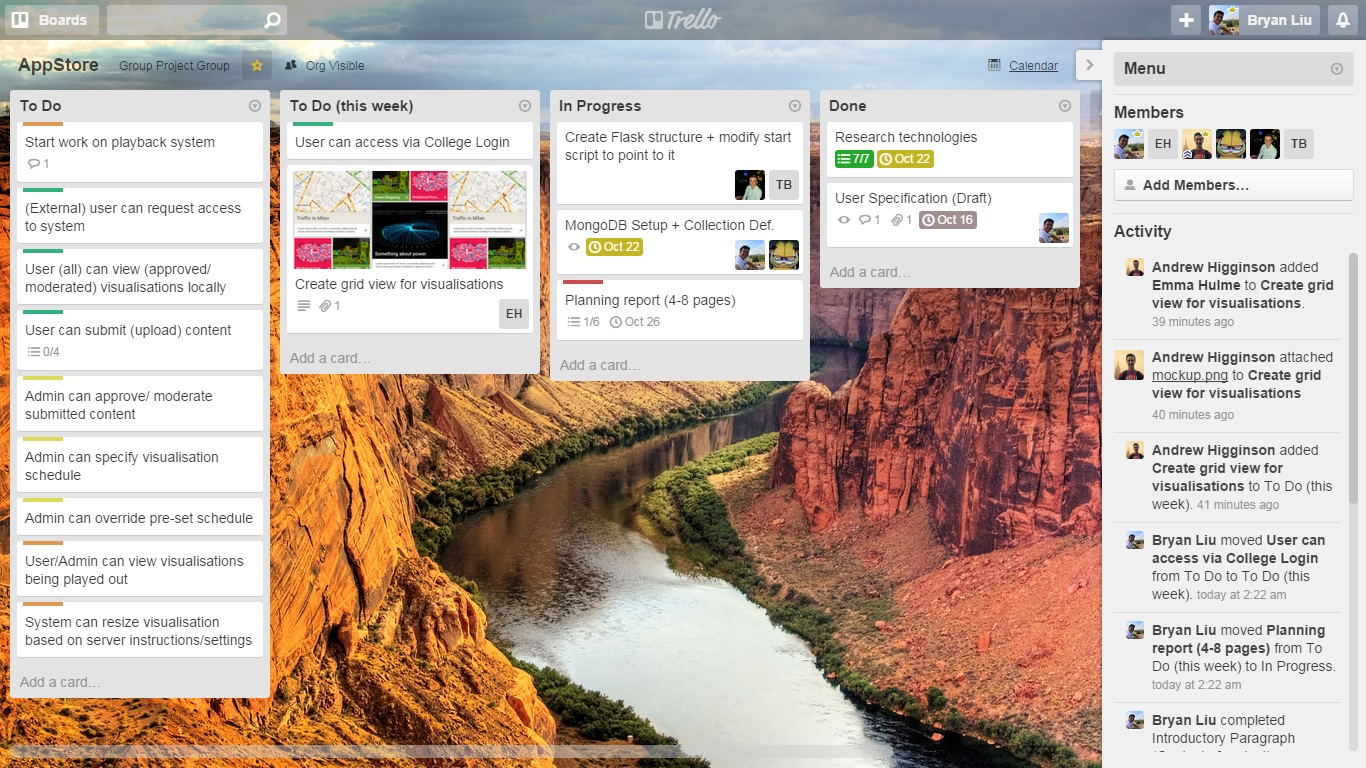
\includegraphics[width = 0.99\textwidth]{./planning/trello.jpg}
   
  \caption{Using Trello to keep track of progress.}
  \label{fig:trello}
\end{figure}

\section{Development Tools}
During the inital phases of our project, we decided on which tools/technologies to use based on our personal preference. For the backend, we decided to use Python with Flask. Members of our team had previously used Ruby on Rails and Python with Django, so we decided to use Flask for interest purposes. To make sure Flask was suitable, the backend team spent time researching additional modules that would allow us to implement future features. We found that Flask met this criterion.

As Bryan and Jackie were more interested in the database side, they chose to use MongoDB as a NoSQL solution. Again, this was based on interest. Bryan used time at the beginning of the project to check that Flask was compatible with MongoDB. 

For the frontend, the AngularJS module was selected. This was chosen as Andrew and Emma wanted to learn a different method of implementing websites in Javascript. 

After a lecture on deployment techniques, the group decided to use Docker. In a group project last year, the backend team had to wait if the frontend was broken to see if particular feature was working. Using Docker and extra virtual machines (created on the department's cloudstack), we can have a separate machine for each feature while it is in development, and have multiple copies of the web server running. Docker allows us to quickly set up the virtual machines via a script, installing any dependencies we need automatically. Although it may be a steep learning curve at the start of our project, Docker will save us a lot of time later. 

We have yet to concretely decide on the best solution for our playout system, as this is relatively independant of the technologies used for the web service. This will be decided in one of our weekly meetings.

As usual, all of our code (including the Docker scripts) will be stored in a group git repository. As a group, we have decided to use branches with a short lifetime. Each minor feature will be implemented on it's own branch, with the master (or trunk) branch used for merging in features only. Merging will take place after the feature is tested on its own branch and vm. 

To deploy the webserver, David has provided us with a Linux vm with root access. Setting up this vm will simply be a case of running our existing scripts with Docker. The playout software will be run on a dedicated computer hooked up to the four projectors, which will be provided by David. 
\end{document}
